\documentclass[aspectratio=169,10pt]{beamer}
\usetheme{Madrid}
\usecolortheme{whale}
\usepackage[utf8]{inputenc}
\usepackage[T1]{fontenc}
\usepackage{tikz}
\usepackage{circuitikz}
\usepackage{array}
\usepackage{colortbl}
\usepackage{multirow}
\usepackage{textcomp}  % For additional symbols
\usetikzlibrary{shapes.geometric, arrows, positioning, fit, backgrounds, calc, patterns}

% Define colors
\definecolor{frontend}{RGB}{245,235,215}  % Beige/cream color
\definecolor{backend}{RGB}{210,225,240}   % Light blue color
\definecolor{alloc}{RGB}{255,0,0}
\definecolor{idqempty}{RGB}{255,0,0}
\definecolor{retiring}{RGB}{0,200,0}
\definecolor{badspec}{RGB}{255,0,0}
\definecolor{frontendbound}{RGB}{150,150,255}
\definecolor{backendbound}{RGB}{255,200,100}
\definecolor{greenbar}{RGB}{150,200,150}
\definecolor{lightgray}{RGB}{220,220,220}

% Custom footer
\setbeamertemplate{footline}{
  \leavevmode%
  \hbox{%
  \begin{beamercolorbox}[wd=.5\paperwidth,ht=2.25ex,dp=1ex,left]{author in head/foot}%
    \usebeamerfont{author in head/foot}\hspace*{2ex}\insertframenumber
  \end{beamercolorbox}%
  \begin{beamercolorbox}[wd=.5\paperwidth,ht=2.25ex,dp=1ex,right]{title in head/foot}%
    \usebeamerfont{title in head/foot}Computer Structure -- Performance Analysis\hspace*{2ex}
  \end{beamercolorbox}}%
  \vskip0pt%
}

\title{Performance Analysis of\\Out-of-Order Cores}
\author{Lihu Rappoport\\{\small Based on Foils by Ahmad Yasin}}
\date{}

\begin{document}

% Slide 1: Title
\begin{frame}
\titlepage
\end{frame}

% Slide 2: Bottleneck Analysis
\begin{frame}{Bottleneck Analysis}
\begin{itemize}
  \item \textbf{Goal:} analyze the HW causes for performance bottlenecks of a given SW running on a processor
  \item \textbf{Method:} classify µop slots at each allocation/rename cycle
  \begin{itemize}
    \item This is the boundary between the Core's frontend (which supplies instructions) and the Core's backend (which consumes instructions)
  \end{itemize}
  \item In the example here we consider a 4-wide machine
\end{itemize}

\vspace{0.2cm}
\begin{center}
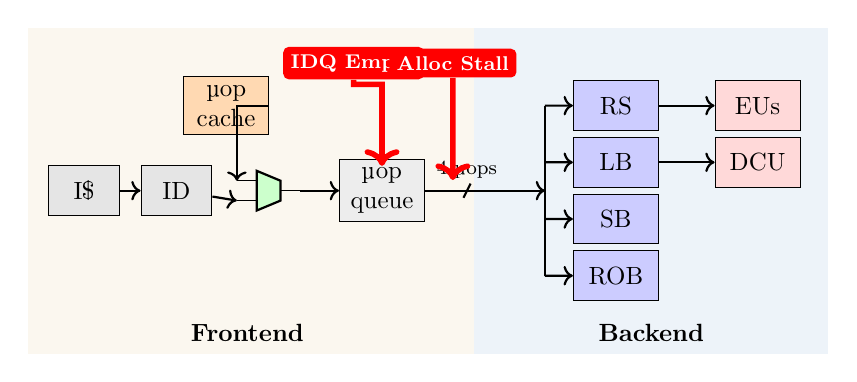
\begin{tikzpicture}[scale=0.9, every node/.style={scale=0.9}]
  % Background shading - drawn first
  \fill[frontend!40] (-0.8,-2.3) rectangle (5.5,2.3);
  \fill[backend!40] (5.5,-2.3) rectangle (10.5,2.3);
  
  % Frontend components
  \node[draw, rectangle, fill=gray!20, minimum width=1cm, minimum height=0.7cm] (icache) at (0,0) {I\$};
  \node[draw, rectangle, fill=gray!20, minimum width=1cm, minimum height=0.7cm] (id) at (1.3,0) {ID};
  
  % µop cache positioned above the mux
  \node[draw, rectangle, fill=orange!30, minimum width=1.2cm, minimum height=0.7cm, align=center] (uopcache) at (2,1.2) {µop\\cache};

  % Mux - selecting between µop cache and ID
  \node[muxdemux, muxdemux def={Lh=1, Rh=0.5, w=0.6, NL=2, NB=0, NT=0}, fill=green!20] (mux) at (2.6,0) {};

  % µop queue (rectangle after mux)
  \node[draw, rectangle, fill=lightgray!50, minimum width=1.2cm, minimum height=0.7cm, align=center] (uopqueue) at (4.2,0) {µop\\queue};

  % Backend components
  \node[draw, rectangle, fill=blue!20, minimum width=1.2cm, minimum height=0.7cm] (rs) at (7.5,1.2) {RS};
  \node[draw, rectangle, fill=blue!20, minimum width=1.2cm, minimum height=0.7cm] (lb) at (7.5,0.4) {LB};
  \node[draw, rectangle, fill=blue!20, minimum width=1.2cm, minimum height=0.7cm] (sb) at (7.5,-0.4) {SB};
  \node[draw, rectangle, fill=blue!20, minimum width=1.2cm, minimum height=0.7cm] (rob) at (7.5,-1.2) {ROB};

  \node[draw, rectangle, fill=red!15, minimum width=1.2cm, minimum height=0.7cm] (eus) at (9.5,1.2) {EUs};
  \node[draw, rectangle, fill=red!15, minimum width=1.2cm, minimum height=0.7cm] (dcu) at (9.5,0.4) {DCU};

  % Arrows
  \draw[->, thick] (icache) -- (id);
  \draw[->, thick] (id) -- (mux.lpin 2);
  \draw[->, thick] (uopcache.east) -| (mux.lpin 1);
  \draw[->, thick] (mux.rpin 1) -- (uopqueue);
  
  % Main connection with 4 µops label
  \draw[->, thick] (uopqueue) -- (6.5,0);
  \draw[thick] (5.35,-0.1) -- (5.45,0.1);  % Small slash through line
  \node[above] at (5.4,0.05) {\footnotesize 4 µops};
  
  % Connect to backend components
  \draw[thick] (6.5,0) -- (6.5,1.2);
  \draw[thick] (6.5,0) -- (6.5,0.4);
  \draw[thick] (6.5,0) -- (6.5,-0.4);
  \draw[thick] (6.5,0) -- (6.5,-1.2);
  \draw[->, thick] (6.5,1.2) -- (rs);
  \draw[->, thick] (6.5,0.4) -- (lb);
  \draw[->, thick] (6.5,-0.4) -- (sb);
  \draw[->, thick] (6.5,-1.2) -- (rob);
  
  % Connect RS and LB to execution units
  \draw[->, thick] (rs) -- (eus);
  \draw[->, thick] (lb) -- (dcu);
  
  % IDQ Empty and Alloc Stall indicators together at the top
  \node[rectangle, rounded corners=2pt, fill=red, text=white, font=\footnotesize\bfseries, inner sep=3pt] (idqempty) at (3.8,1.8) {IDQ Empty};
  \node[rectangle, rounded corners=2pt, fill=red, text=white, font=\footnotesize\bfseries, inner sep=3pt] (allocstall) at (5.2,1.8) {Alloc Stall};
  
  % Arrow from IDQ Empty pointing to µop queue
  \draw[->, line width=2pt, red] (idqempty.south) -- (3.8,1.5) -- (4.2,1.5) -- (4.2,0.35);
  
  % Arrow from Alloc Stall pointing to the 4 µops line
  \draw[->, line width=2pt, red] (allocstall.south) -- (5.2,1.5) -- (5.2,0.15);
  
  % Labels
  \node[font=\normalsize\bfseries] at (2.3,-2) {Frontend};
  \node[font=\normalsize\bfseries] at (8,-2) {Backend};
\end{tikzpicture}
\end{center}
\end{frame}

% Slide 3: Allocation Stall
\begin{frame}{Allocation Stall}
\begin{itemize}
  \item \textbf{Allocation is done all-or-none}
  \begin{itemize}
    \item If in a given cycle the frontend supplies n$\leq$4 µops, and the backend does not have room for all n µops (e.g., the RS has fewer than n free entries)
    \begin{itemize}
      \item Allocation is stalled for the cycle, and no µop is allocated in that cycle
      \item Stall is removed once the backend has room for all the µops supplied by the frontend in the cycle (up to 4 µops / cycle in the 4-wide machine used here)
    \end{itemize}
  \end{itemize}
\end{itemize}

\vspace{0.2cm}
\begin{center}
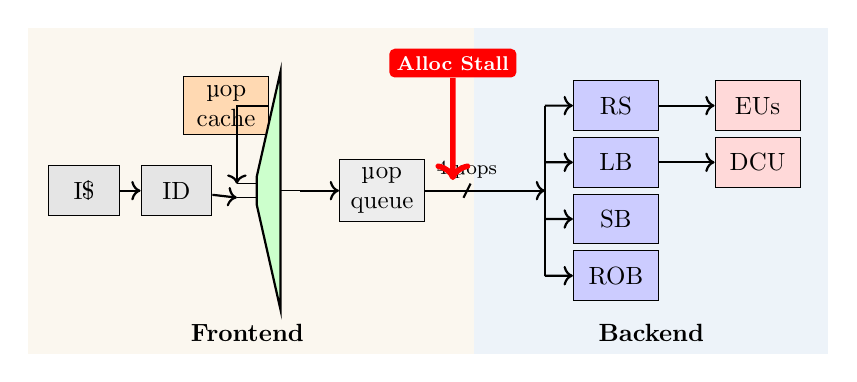
\begin{tikzpicture}[scale=0.9, every node/.style={scale=0.9}]
  % Background shading - drawn first
  \fill[frontend!40] (-0.8,-2.3) rectangle (5.5,2.3);
  \fill[backend!40] (5.5,-2.3) rectangle (10.5,2.3);
  
  % Frontend components
  \node[draw, rectangle, fill=gray!20, minimum width=1cm, minimum height=0.7cm] (icache) at (0,0) {I\$};
  \node[draw, rectangle, fill=gray!20, minimum width=1cm, minimum height=0.7cm] (id) at (1.3,0) {ID};
  
  % µop cache positioned above the mux
  \node[draw, rectangle, fill=orange!30, minimum width=1.2cm, minimum height=0.7cm, align=center] (uopcache) at (2,1.2) {µop\\cache};

  % Mux - selecting between µop cache and ID
  \node[muxdemux, muxdemux def={Lh=0.7, w=0.6, NL=2, NB=0, NT=0}, fill=green!20] (mux) at (2.6,0) {};

  % µop queue (rectangle after mux)
  \node[draw, rectangle, fill=lightgray!50, minimum width=1.2cm, minimum height=0.7cm, align=center] (uopqueue) at (4.2,0) {µop\\queue};

  % Backend components
  \node[draw, rectangle, fill=blue!20, minimum width=1.2cm, minimum height=0.7cm] (rs) at (7.5,1.2) {RS};
  \node[draw, rectangle, fill=blue!20, minimum width=1.2cm, minimum height=0.7cm] (lb) at (7.5,0.4) {LB};
  \node[draw, rectangle, fill=blue!20, minimum width=1.2cm, minimum height=0.7cm] (sb) at (7.5,-0.4) {SB};
  \node[draw, rectangle, fill=blue!20, minimum width=1.2cm, minimum height=0.7cm] (rob) at (7.5,-1.2) {ROB};

  \node[draw, rectangle, fill=red!15, minimum width=1.2cm, minimum height=0.7cm] (eus) at (9.5,1.2) {EUs};
  \node[draw, rectangle, fill=red!15, minimum width=1.2cm, minimum height=0.7cm] (dcu) at (9.5,0.4) {DCU};

  % Arrows
  \draw[->, thick] (icache) -- (id);
  \draw[->, thick] (id) -- (mux.lpin 2);
  \draw[->, thick] (uopcache.east) -| (mux.lpin 1);
  \draw[->, thick] (mux.rpin 1) -- (uopqueue);
  
  % Main connection with 4 µops label
  \draw[->, thick] (uopqueue) -- (6.5,0);
  \draw[thick] (5.35,-0.1) -- (5.45,0.1);  % Small slash through line
  \node[above] at (5.4,0.05) {\footnotesize 4 µops};
  
  % Connect to backend components
  \draw[thick] (6.5,0) -- (6.5,1.2);
  \draw[thick] (6.5,0) -- (6.5,0.4);
  \draw[thick] (6.5,0) -- (6.5,-0.4);
  \draw[thick] (6.5,0) -- (6.5,-1.2);
  \draw[->, thick] (6.5,1.2) -- (rs);
  \draw[->, thick] (6.5,0.4) -- (lb);
  \draw[->, thick] (6.5,-0.4) -- (sb);
  \draw[->, thick] (6.5,-1.2) -- (rob);
  
  % Connect RS and LB to execution units
  \draw[->, thick] (rs) -- (eus);
  \draw[->, thick] (lb) -- (dcu);
  
  % Alloc Stall indicator (only this one for slide 3)
  \node[rectangle, rounded corners=2pt, fill=red, text=white, font=\footnotesize\bfseries, inner sep=3pt] (allocstall) at (5.2,1.8) {Alloc Stall};
  \draw[->, line width=2pt, red] (allocstall.south) -- (5.2,1.5) -- (5.2,0.15);
  
  % Labels
  \node[font=\normalsize\bfseries] at (2.3,-2) {Frontend};
  \node[font=\normalsize\bfseries] at (8,-2) {Backend};
\end{tikzpicture}
\end{center}
\end{frame}

% Slide 4: Allocation Slot Classification
\begin{frame}{Allocation Slot Classification}
\begin{itemize}
  \item \textbf{Backend-bound:} for a cycle with a back-end stall (allocation stall)
  \begin{itemize}
    \item All 4 allocation slots are counted as backend bound
  \end{itemize}
  \item \textbf{Frontend-bound:} in a cycle without a back-end stall
  \begin{itemize}
    \item If the frontend provides n<4 µops, this cycle is bound by fronted supply:\\
    it has (4 - n) frontend bound allocation slots
  \end{itemize}
  \item \textbf{Retiring:} the number ($\leq$4) of µops in the cycle which \underline{eventually} retire (counting done at retire)
  \item \textbf{Bad speculation:} the number ($\leq$4) of µops in the cycle which \underline{eventually} do not retire\\
  (due to some bad speculation, e.g., jump misprediction – counting done at recovery/reclamation)
\end{itemize}

\vspace{0.3cm}
\begin{center}
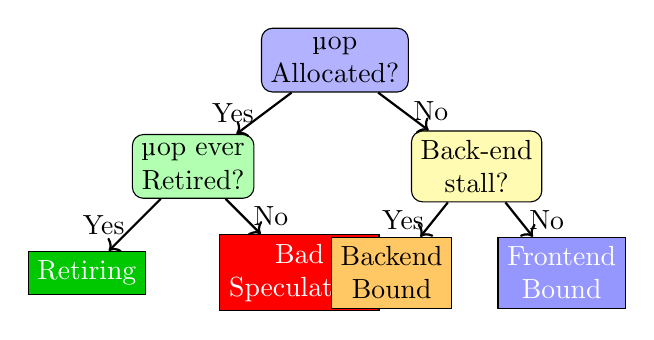
\begin{tikzpicture}[scale=0.9]
  % Decision tree
  \node[draw, rectangle, fill=blue!30, rounded corners, align=center] (root) at (0,0) {µop\\Allocated?};
  
  \node[draw, rectangle, fill=green!30, rounded corners, align=center] (retired) at (-2,-1.5) {µop ever\\Retired?};
  \node[draw, rectangle, fill=yellow!30, rounded corners, align=center] (stall) at (2,-1.5) {Back-end\\stall?};
  
  \node[draw, rectangle, fill=retiring, text=white] (retiring) at (-3.5,-3) {Retiring};
  \node[draw, rectangle, fill=badspec, text=white, align=center] (badspec) at (-0.5,-3) {Bad\\Speculation};
  \node[draw, rectangle, fill=backendbound, align=center] (backend) at (0.8,-3) {Backend\\Bound};
  \node[draw, rectangle, fill=frontendbound, text=white, align=center] (frontend) at (3.2,-3) {Frontend\\Bound};
  
  % Arrows
  \draw[->, thick] (root) -- node[left] {Yes} (retired);
  \draw[->, thick] (root) -- node[right] {No} (stall);
  \draw[->, thick] (retired) -- node[left] {Yes} (retiring);
  \draw[->, thick] (retired) -- node[right] {No} (badspec);
  \draw[->, thick] (stall) -- node[left] {Yes} (backend);
  \draw[->, thick] (stall) -- node[right] {No} (frontend);
\end{tikzpicture}
\end{center}
\end{frame}

% Slide 5: Per Cycle Classification (1)
\begin{frame}{Per Cycle Classification (1)}
\begin{itemize}
  \item Each column represents an allocation cycle
\end{itemize}

\begin{center}
\begin{tabular}{|l|c|}
\hline
\rowcolor{red!20} Cycle & 1 \\
\hline
\rowcolor{red!20} Back-end Stall & 0 \\
\hline
\rowcolor{greenbar!50} Alloc Slot 0 & - \\
\hline
\rowcolor{greenbar!50} Alloc Slot 1 & - \\
\hline
\rowcolor{greenbar!50} Alloc Slot 2 & - \\
\hline
\rowcolor{greenbar!50} Alloc Slot 3 & - \\
\hline
\rowcolor{frontendbound} Frontend Bound & 4 \\
\hline
\rowcolor{backendbound} Backend Bound & \\
\hline
\rowcolor{retiring} Retiring & \\
\hline
\rowcolor{badspec} \textcolor{white}{Bad Speculation} & \\
\hline
\end{tabular}
\end{center}

\begin{itemize}
  \item No Allocation stall
  \item No µop is supplied by frontend
  \item All 4 slots count as frontend bound
\end{itemize}
\end{frame}

% Slide 6: Per Cycle Classification (2)
\begin{frame}{Per Cycle Classification (2)}
\begin{itemize}
  \item Each column represents an allocation cycle
\end{itemize}

\begin{center}
\begin{tabular}{|l|c|c|}
\hline
\rowcolor{red!20} Cycle & 1 & 2 \\
\hline
\rowcolor{red!20} Back-end Stall & 0 & 0 \\
\hline
\rowcolor{greenbar!50} Alloc Slot 0 & & v \\
\hline
\rowcolor{greenbar!50} Alloc Slot 1 & & v \\
\hline
\rowcolor{greenbar!50} Alloc Slot 2 & & - \\
\hline
\rowcolor{greenbar!50} Alloc Slot 3 & & - \\
\hline
\rowcolor{frontendbound} Frontend Bound & & 2 \\
\hline
\rowcolor{backendbound} Backend Bound & & \\
\hline
\rowcolor{retiring} Retiring & & 2 \\
\hline
\rowcolor{badspec} \textcolor{white}{Bad Speculation} & & \\
\hline
\end{tabular}
\end{center}

\begin{itemize}
  \item No Allocation stall
  \item 2 µops are supplied by frontend
  \item 2 slots are frontend bound, and 2 slots are retiring
\end{itemize}
\end{frame}

% Slide 7: Per Cycle Classification (3)
\begin{frame}{Per Cycle Classification (3)}
\begin{itemize}
  \item Each column represents an allocation cycle
\end{itemize}

\begin{center}
\begin{tabular}{|l|c|c|c|}
\hline
\rowcolor{red!20} Cycle & 1 & 2 & 3 \\
\hline
\rowcolor{red!20} Back-end Stall & 0 & 0 & 1 \\
\hline
\rowcolor{greenbar!50} Alloc Slot 0 & & v & - \\
\hline
\rowcolor{greenbar!50} Alloc Slot 1 & & v & - \\
\hline
\rowcolor{greenbar!50} Alloc Slot 2 & & - & - \\
\hline
\rowcolor{greenbar!50} Alloc Slot 3 & & - & - \\
\hline
\rowcolor{frontendbound} Frontend Bound & & & \\
\hline
\rowcolor{backendbound} Backend Bound & & & 4 \\
\hline
\rowcolor{retiring} Retiring & & 2 & \\
\hline
\rowcolor{badspec} \textcolor{white}{Bad Speculation} & & & \\
\hline
\end{tabular}
\end{center}

\begin{itemize}
  \item Allocation stall
  \item 4 slots are backend bound
\end{itemize}
\end{frame}

% Slide 8: Per Cycle Classification (4)
\begin{frame}{Per Cycle Classification (4)}
\begin{itemize}
  \item Each column represents an allocation cycle
\end{itemize}

\begin{center}
\begin{tabular}{|l|c|c|c|c|}
\hline
\rowcolor{red!20} Cycle & 1 & 2 & 3 & 4 \\
\hline
\rowcolor{red!20} Back-end Stall & 0 & 0 & 1 & 0 \\
\hline
\rowcolor{greenbar!50} Alloc Slot 0 & & v & & v \\
\hline
\rowcolor{greenbar!50} Alloc Slot 1 & & v & & \textcolor{red}{v} \\
\hline
\rowcolor{greenbar!50} Alloc Slot 2 & & - & & \textcolor{red}{v} \\
\hline
\rowcolor{greenbar!50} Alloc Slot 3 & & - & & \textcolor{red}{v} \\
\hline
\rowcolor{frontendbound} Frontend Bound & & & & 0 \\
\hline
\rowcolor{backendbound} Backend Bound & & & & 0 \\
\hline
\rowcolor{retiring} Retiring & & 2 & & 1 \\
\hline
\rowcolor{badspec} \textcolor{white}{Bad Speculation} & & & & \textcolor{white}{3} \\
\hline
\end{tabular}
\end{center}

\begin{itemize}
  \item No Allocation stall
  \item 4 µops are supplied by frontend
  \item 1 slot retires, and 3 slots are flushed due to bad speculation
\end{itemize}
\end{frame}

% Slide 9: Per Cycle Classification (5)
\begin{frame}{Per Cycle Classification (5)}
\begin{itemize}
  \item Each column represents an allocation cycle
\end{itemize}

\begin{center}
\begin{tabular}{|l|c|c|c|c|c|}
\hline
\rowcolor{red!20} Cycle & 1 & 2 & 3 & 4 & 5 \\
\hline
\rowcolor{red!20} Back-end Stall & 0 & 0 & 1 & 0 & 0 \\
\hline
\rowcolor{greenbar!50} Alloc Slot 0 & & v & & v & v \\
\hline
\rowcolor{greenbar!50} Alloc Slot 1 & & v & & \textcolor{red}{v} & v \\
\hline
\rowcolor{greenbar!50} Alloc Slot 2 & & - & & \textcolor{red}{v} & \textcolor{red}{v} \\
\hline
\rowcolor{greenbar!50} Alloc Slot 3 & & - & & \textcolor{red}{v} & - \\
\hline
\rowcolor{frontendbound} Frontend Bound & & & & 0 & 1 \\
\hline
\rowcolor{backendbound} Backend Bound & & & & 0 & 0 \\
\hline
\rowcolor{retiring} Retiring & & 2 & & 1 & 2 \\
\hline
\rowcolor{badspec} \textcolor{white}{Bad Speculation} & & & & \textcolor{white}{3} & \textcolor{white}{1} \\
\hline
\end{tabular}
\end{center}

\begin{itemize}
  \item No Allocation stall
  \item 3 µops are supplied by frontend
  \item 1 slots frontend bound, 2 slot retire, and 1 slot bad speculation
\end{itemize}
\end{frame}

% Slide 10: Bottleneck Summary
\begin{frame}{Bottleneck Summary}
\begin{itemize}
  \item Each column represents an allocation cycle
\end{itemize}

\begin{center}
\begin{tabular}{|l|c|c|c|c|c||c|c|}
\hline
\rowcolor{red!20} Cycle & 1 & 2 & 3 & 4 & 5 & & \\
\hline
\rowcolor{red!20} Back-end Stall & 0 & 0 & 1 & 0 & 0 & & \\
\hline
\rowcolor{greenbar!50} Alloc Slot 0 & - & v & - & v & v & & \\
\hline
\rowcolor{greenbar!50} Alloc Slot 1 & - & v & - & \textcolor{red}{v} & v & & \\
\hline
\rowcolor{greenbar!50} Alloc Slot 2 & - & - & - & \textcolor{red}{v} & \textcolor{red}{v} & & \\
\hline
\rowcolor{greenbar!50} Alloc Slot 3 & - & - & - & \textcolor{red}{v} & - & & \\
\hline
\rowcolor{frontendbound} Frontend Bound & 4 & 2 & & 0 & 1 & 7 & 7/20 = 35\% \\
\hline
\rowcolor{backendbound} Backend Bound & & & 4 & 0 & 0 & 4 & 4/20 = 20\% \\
\hline
\rowcolor{retiring} Retiring & & 2 & & 1 & 2 & 5 & 5/20 = 25\% \\
\hline
\rowcolor{badspec} \textcolor{white}{Bad Speculation} & & & & \textcolor{white}{3} & \textcolor{white}{1} & \textcolor{white}{4} & \textcolor{white}{4/20 = 20\%} \\
\hline
\end{tabular}
\end{center}

\begin{itemize}
  \item IPC = 5 µops / 5 cycles = 1
  \begin{itemize}
    \item Note that in this 4-wide machine, the maximum IPC is 4, which would have been achieved if all 20 allocation slots during the run contained retiring µops
  \end{itemize}
\end{itemize}
\end{frame}

% Slide 11: The Top-Down Hierarchy
\begin{frame}{The Top-Down Hierarchy}
\begin{itemize}
  \item Performance counters are provided to capture the various events
  \begin{itemize}
    \item Analysis tools use the performance counters to build the top-down hierarchy
  \end{itemize}
\end{itemize}

\vspace{0.2cm}
\begin{center}
\resizebox{0.9\textwidth}{!}{
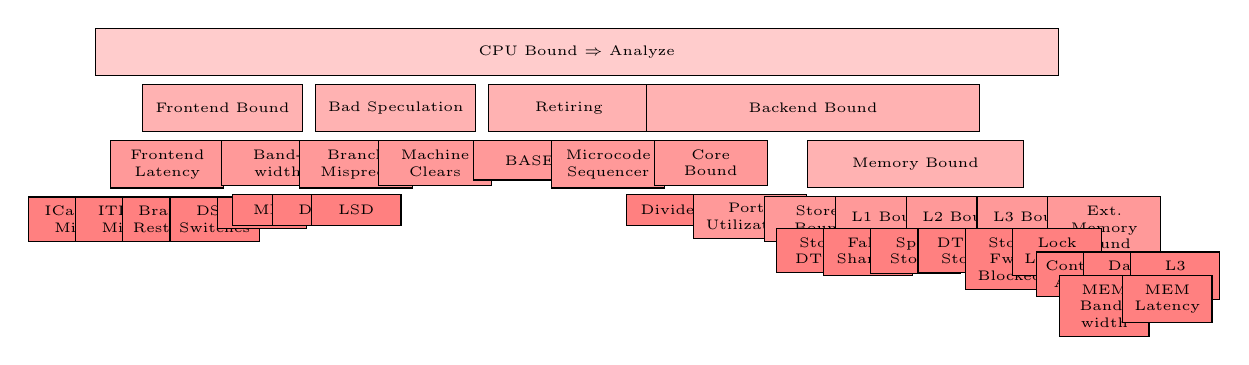
\begin{tikzpicture}[
  box/.style={rectangle, draw, fill=red!30, text width=1.8cm, text centered, minimum height=0.6cm, font=\tiny, align=center},
  smallbox/.style={rectangle, draw, fill=red!40, text width=1.2cm, text centered, minimum height=0.5cm, font=\tiny, align=center},
  tinybox/.style={rectangle, draw, fill=red!50, text width=0.9cm, text centered, minimum height=0.4cm, font=\tiny, align=center}
]
  % Root
  \node[box, text width=12cm, fill=red!20, align=center] (root) at (0,0) {CPU Bound $\Rightarrow$ Analyze};
  
  % Level 1
  \node[box, below=0.1cm of root, xshift=-4.5cm] (frontend) {Frontend Bound};
  \node[box, below=0.1cm of root, xshift=-2.3cm] (badspec) {Bad Speculation};
  \node[box, below=0.1cm of root, xshift=-0.1cm] (retiring) {Retiring};
  \node[box, text width=4cm, below=0.1cm of root, xshift=3cm, align=center] (backend) {Backend Bound};
  
  % Level 2 - Frontend
  \node[smallbox, below=0.1cm of frontend, xshift=-0.7cm] (latency) {Frontend Latency};
  \node[smallbox, below=0.1cm of frontend, xshift=0.7cm] (bandwidth) {Band-width};
  
  % Level 2 - Bad Spec
  \node[smallbox, below=0.1cm of badspec, xshift=-0.5cm] (branch) {Branch Mispred.};
  \node[smallbox, below=0.1cm of badspec, xshift=0.5cm] (machine) {Machine Clears};
  
  % Level 2 - Retiring
  \node[smallbox, below=0.1cm of retiring, xshift=-0.5cm] (base) {BASE};
  \node[smallbox, below=0.1cm of retiring, xshift=0.5cm] (microcode) {Microcode Sequencer};
  
  % Level 2 - Backend
  \node[smallbox, below=0.1cm of backend, xshift=-1.3cm] (core) {Core Bound};
  \node[box, text width=2.5cm, below=0.1cm of backend, xshift=1.3cm, align=center] (memory) {Memory Bound};
  
  % Level 3 - Frontend details
  \node[tinybox, below=0.1cm of latency, xshift=-1.2cm, font=\tiny] {ICache Miss};
  \node[tinybox, below=0.1cm of latency, xshift=-0.6cm, font=\tiny] {ITLB Miss};
  \node[tinybox, below=0.1cm of latency, xshift=0cm, font=\tiny] {Branch Resteers};
  \node[tinybox, below=0.1cm of latency, xshift=0.6cm, font=\tiny] {DSB Switches};
  \node[tinybox, below=0.1cm of latency, xshift=1.2cm, font=\tiny] {LCP};
  \node[tinybox, below=0.1cm of bandwidth, font=\tiny] {MITE};
  \node[tinybox, below=0.1cm of bandwidth, xshift=0.5cm, font=\tiny] {DSB};
  \node[tinybox, below=0.1cm of bandwidth, xshift=1cm, font=\tiny] {LSD};
  
  % Level 3 - Backend details
  \node[tinybox, below=0.1cm of core, xshift=-0.5cm] {Divider};
  \node[smallbox, below=0.1cm of core, xshift=0.5cm] {Ports Utilization};
  
  \node[smallbox, below=0.1cm of memory, xshift=-1.2cm] {Stores Bound};
  \node[smallbox, below=0.1cm of memory, xshift=-0.3cm] {L1 Bound};
  \node[smallbox, below=0.1cm of memory, xshift=0.6cm] {L2 Bound};
  \node[smallbox, below=0.1cm of memory, xshift=1.5cm] {L3 Bound};
  \node[smallbox, below=0.1cm of memory, xshift=2.4cm] {Ext. Memory Bound};
  
  % Level 4 - More details
  \node[tinybox, below=0.5cm of memory, xshift=-1.2cm, font=\tiny] {Store DTLB};
  \node[tinybox, below=0.5cm of memory, xshift=-0.6cm, font=\tiny] {False Sharing};
  \node[tinybox, below=0.5cm of memory, xshift=0cm, font=\tiny] {Split Stores};
  \node[tinybox, below=0.5cm of memory, xshift=0.6cm, font=\tiny] {DTLB Store};
  \node[tinybox, below=0.5cm of memory, xshift=1.2cm, font=\tiny] {Store Fwd. Blocked};
  \node[tinybox, below=0.5cm of memory, xshift=1.8cm, font=\tiny] {Lock Latency};
  
  \node[tinybox, below=0.8cm of memory, xshift=2.1cm, font=\tiny] {Contested Access};
  \node[tinybox, below=0.8cm of memory, xshift=2.7cm, font=\tiny] {Data Sharing};
  \node[tinybox, below=0.8cm of memory, xshift=3.3cm, font=\tiny] {L3 Latency};
  
  \node[tinybox, below=1.1cm of memory, xshift=2.4cm, font=\tiny] {MEM Bandwidth};
  \node[tinybox, below=1.1cm of memory, xshift=3.2cm, font=\tiny] {MEM Latency};
\end{tikzpicture}
}
\end{center}
\end{frame}

\end{document}